\documentclass[11pt,a4paper]{article}

\usepackage[T1]{fontenc}
\usepackage[utf8]{inputenc}
\usepackage{lmodern}
\usepackage{microtype}
\usepackage[margin=1in]{geometry}
\usepackage{amsmath,amssymb,amsthm}
\usepackage{booktabs}
\usepackage{array}
\usepackage{enumitem}
\usepackage{tikz}
\usetikzlibrary{arrows.meta,positioning,calc}
\usepackage{url}
\usepackage[hidelinks]{hyperref}

\setlist[enumerate]{itemsep=0.25em,topsep=0.4em}
\setlist[itemize]{itemsep=0.2em,topsep=0.35em}

\newcommand{\valid}[1]{\lfloor #1 \rfloor}
\newcommand{\Nec}{\Box}
\newcommand{\Pos}{\Diamond}
\newcommand{\exE}{\exists^{E}}
\newcommand{\allE}{\forall^{E}}
\newcommand{\necImp}{\supset_{N}}
\newcommand{\lean}[1]{\texttt{#1}}

\newtheorem{theorem}{Theorem}
\newtheorem{lemma}[theorem]{Lemma}
\newtheorem{proposition}[theorem]{Proposition}
\theoremstyle{definition}
\newtheorem{definition}[theorem]{Definition}
\theoremstyle{remark}
\newtheorem{remark}[theorem]{Remark}

\title{Where the Box Sits:\\
Ax1Gen and G\"odel's Theorem Th3 in S4}
\author{Drew Arrowood}
\date{September 2026}

\begin{document}
\maketitle

\begin{abstract}
Benzm\"uller and Scott leave open whether Theorem Th3 of their actualist
Figure~7---possible existence of a God-like being implies necessary
existence, with \(P(G)\) derived from the generalized conjunction axiom
Ax1Gen---is provable in S4.
Two Lean~4 theorems decide that question, and they decide it in opposite
directions, according to a single scope.
Read literally, as in the Archive of Formal Proofs, Ax1Gen tests positivity
of a collection \(\Phi\) at the current world and reads \(\Phi\) again under
a box.
That split forces the accessibility relation to be symmetric, so Th3 holds
in S4 with no reflexivity or transitivity hypothesis.
Two repairs that put the scopes back together---positivity inside the box,
or a world-invariant \(\Phi\)---still yield the lemma \(P(G)\), do not force
symmetry, and fail on a two-world S4 chain.
The open question is settled entirely by where Ax1Gen looks.
\end{abstract}

\section{A footnote, a notebook, and an \texttt{oops}}
\label{sec:hook}

Around 1970 Kurt G\"odel wrote down, in a page and a half of symbols, a modal
version of the ontological argument
\cite{goedel1995}.
The first axiom says that the conjunction of two positive properties is
positive.
A footnote extends the axiom from two summands to any number of them: the
conjunction of a collection of positive properties is itself positive.
Dana Scott, working from a copy G\"odel allowed him to make, rearranged the
package \cite{scott2004notes,sobel1987,sobel2004}.
In Scott's notes the generalized conjunction is replaced by a direct
postulate that being God-like is positive.
Scott also inserts a conjunct into the definition of essence, requiring that
the essential property actually hold of the individual, and he takes necessary
existence to be positive.
That last change is the one that keeps the notes off the inconsistent reading
of the unrepaired manuscript.

Jordan Howard Sobel later showed that Scott's premises collapse modality:
whatever is true is necessarily true \cite{sobel1987,sobel2004}.
The collapse has since been machine-checked, and so have repairs in the
spirit of Anderson and of Fitting
\cite{anderson1990,fitting2002,benzmuellerFuenmayor2020}.
Separately, the passage from ``possibly God-like'' to ``necessarily
God-like'' on the Scott side needs symmetry of accessibility, the modal axiom
B, and does not need the rest of S5 \cite{kanckos2017}.
None of that is the question of this note.
Those facts are recorded again in Section~\ref{sec:related} only so that they
are not mistaken for the two theorems below.

The question comes from a return to the footnote.
Christoph Benzm\"uller and Dana Scott, in the \emph{Monatshefte f\"ur
Mathematik} \cite{benzmuellerScott2025}, and in the matching Archive of Formal
Proofs entry \cite{afpNotes2025}, study G\"odel's own generalized conjunction
as an axiom they call Ax1Gen.
Positivity of being God-like is not assumed.
It is lemma~L, derived from Ax1Gen.
Essence keeps Scott's extra conjunct.
Individual quantifiers in the argument are actualist: an existence predicate
says who is around at a world.
In their Figure~7, Theorem Th3 is
\[
  \valid{\Pos(\exE x.\, G x) \supset \Nec(\exE y.\, G y)}.
\]
In the S5 embedding the proof uses symmetry of the accessibility relation and
nothing else from S5.
The theory \lean{GoedelVariantHOML2inS4} repeats the same non-logical axioms
over an S4 frame (reflexive and transitive, symmetry not assumed) and leaves
Th3 as \lean{oops}, with the comment ``Open problem''.
The header of that theory says that the proof of Th3 fails in S4.
Figure~8, which repairs the argument by changing necessary inclusion instead
of essence, has the same open \lean{oops} in
\lean{GoedelVariantHOML3inS4}.
The authors' formalization reports neither an S4 proof nor an S4 countermodel.

This note records two theorems already checked in Lean~4, in the repository
described in the acknowledgement.
They answer the open problem for the literal AFP axiom, and they answer it
again after two repairs of a scope that the footnote does not ask for.
The literal reading proves Th3.
The repairs refute it in S4.
Which answer one gets is exactly the source/successor split in Ax1Gen.

\section{Figure 7, as formalized}
\label{sec:fig7}

Worlds form a type \(W\), individuals a type \(\mathit{Ind}\), and
accessibility is a relation \(R\) on \(W\).
A world-proposition is a map \(W \to \mathsf{Prop}\).
A property is a map \(\mathit{Ind} \to W \to \mathsf{Prop}\), individual first
and world second, matching the AFP type \(e \Rightarrow i \Rightarrow
\mathsf{bool}\).
Positivity \(P\) is a world-relative predicate on properties.
Necessity and possibility are the usual quantifications along \(R\):
\[
  (\Nec\varphi)\,w \;\equiv\; \forall v.\; R\,w\,v \to \varphi\,v,
  \qquad
  (\Pos\varphi)\,w \;\equiv\; \exists v.\; R\,w\,v \land \varphi\,v.
\]
Validity \(\valid{\varphi}\) means \(\varphi\) holds at every world.

An existence predicate \(\mathit{ex} : \mathit{Ind} \to W \to \mathsf{Prop}\)
plays the role of the AFP constant \(\mathit{existsAt}\).
The outer type of individuals is fixed.
Who exists may vary.
Actualist quantifiers are the restrictions
\[
  (\allE y.\, \varphi\,y)\,w
    \;\equiv\; \forall y.\; \mathit{ex}\,y\,w \to \varphi\,y\,w,
  \qquad
  (\exE y.\, \varphi\,y)\,w
    \;\equiv\; \exists y.\; \mathit{ex}\,y\,w \land \varphi\,y\,w.
\]
Quantifiers over properties stay possibilist: they range over every map
\(\mathit{Ind} \to W \to \mathsf{Prop}\).

God-likeness, necessary inclusion, essence, and necessary existence are the
Figure~7 clauses.
Writing \(\varphi \mathbin{\cdot} \psi\) for the pointwise conjunction of
properties and \(\sim\varphi\) for pointwise negation:
\begin{align*}
  G\,x &\;\equiv\; \forall \varphi.\; P\,\varphi \supset \varphi\,x,\\
  \varphi \necImp \psi
    &\;\equiv\; \Nec(\allE y.\, \varphi\,y \supset \psi\,y),\\
  \varphi \mathbin{\mathrm{Ess.}} x
    &\;\equiv\; \varphi\,x \land
      (\forall \psi.\; \psi\,x \supset (\varphi \necImp \psi)),\\
  E\,x &\;\equiv\; \forall \varphi.\;
      (\varphi \mathbin{\mathrm{Ess.}} x) \supset \Nec(\exE z.\, \varphi\,z).
\end{align*}
The AFP binder in the last clause shadows \(x\); the Lean definition uses a
fresh variable, which is the same formula.
The axioms, all under validity, are Ax1 (binary conjunction), Ax2a (exclusive
disjunction of \(P\,\varphi\) and \(P(\sim\varphi)\)), Ax2b
(\(P\,\varphi \supset \Nec P\,\varphi\)), Ax3 (\(P\,E\)), and Ax4 (a positive
property passes positivity along \(\necImp\)).
Ax1 is part of the package and holds in the one-world model of
Section~\ref{sec:th1}.
Th3 does not use it.
The AFP proof of Th3 does not use it either.

The footnote becomes two abbreviations and one axiom.
\begin{align*}
  \mathrm{PosProps}\,\Phi
    &\;\equiv\; \forall \varphi.\; \Phi\,\varphi \supset P\,\varphi,\\
  \mathrm{ConjOfPropsFrom}\,\varphi\,\Phi
    &\;\equiv\; \Nec\bigl(\allE z.\;
        \varphi\,z \leftrightarrow
        (\forall \psi.\; \Phi\,\psi \supset \psi\,z)\bigr),\\
  \mathrm{Ax1Gen}
    &\;\equiv\; \valid{(\mathrm{PosProps}\,\Phi \land
        \mathrm{ConjOfPropsFrom}\,\varphi\,\Phi) \supset P\,\varphi}.
\end{align*}
Both \(\Phi\) and \(\varphi\) are universally quantified.
This is the text of \lean{GoedelVariantHOML2} and of
\lean{GoedelVariantHOML2inS4}.
Lemma~L is \(\valid{P\,G}\), obtained by feeding Ax1Gen the collection of
properties that are positive at the world of evaluation.
It is a lemma, not an axiom.
Scott's later A3 postulates that same sentence outright
\cite{scott2004notes}.
The two packages are different, and Section~\ref{sec:related} is there to keep
them apart.

In the S5 theory, Th3 is proved from Th2 by the three steps the AFP script
writes down: existence of a God-like being implies necessary existence; the
diamond of the antecedent is therefore a diamond of a box; symmetry turns
that diamond-box back into a box.
The Lean theorem \lean{th3\_of\_symmetric} is that argument, with the witness
individual written out.
Reflexivity is not used.

\section{What the encoding is}
\label{sec:encoding}

The development is a shallow embedding in Lean~4 \cite{demouraUllrich2021},
with no Mathlib library.
Hypotheses are propositions, passed as arguments.
There is no Lean \lean{axiom} declaration anywhere in the repository.
The host logic is the ordinary Lean kernel.
Where a proof uses classical reasoning, \lean{\#print axioms} says so
(Section~\ref{sec:kernel}).
Isabelle/HOL is classical \cite{nipkow2002}, so that use of classical logic
matches the host logic of the AFP entry.
It is still a different host.

The departures from the AFP text are these.

\begin{center}
\small
\begin{tabular}{@{}p{0.46\textwidth}p{0.48\textwidth}@{}}
\toprule
AFP & This Lean development \\
\midrule
Isabelle/HOL \textsf{bool} &
  Lean \textsf{Prop}.
  Classical steps are exactly the ones whose axiom list contains
  \lean{Classical.choice}. \\
\(\valid{\psi} \equiv \forall w.\, \psi\,w\) &
  The definition \lean{valid}. \\
\(\mathit{existsAt} : e \Rightarrow \sigma\) &
  \(\mathit{ex} : \mathit{Ind} \to W \to \mathsf{Prop}\).
  A fixed outer type, with existence varying by world, is how the AFP file
  represents varying domains. \\
Property quantifiers are HOL \(\forall\) over functions \(e \Rightarrow \sigma\) &
  Lean \(\forall\) over functions \(\mathit{Ind} \to W \to \mathsf{Prop}\).
  Comprehension is full, as in their impredicative Ax1Gen. \\
Figure~8 writes \(\varphi \neq (\lambda x.\, \bot)\), which is extensional
inequality of HOL functions &
  \lean{neBot}: \(\neg \forall x\,w.\, \varphi\,x\,w \leftrightarrow \mathsf{False}\).
  The symmetry proof supplies a pointwise witness.
  Lean's intensional \(\varphi \neq \bot\) is a different statement, and it is
  not the one used. \\
Deep surface syntax, Leibniz equality inside the object logic, Nitpick &
  Absent.
  The one-world model of Section~\ref{sec:th1} is the cardinality-one shape
  Nitpick reported, rebuilt by hand. \\
\bottomrule
\end{tabular}
\end{center}

World-relative \(P\), actualist individual quantifiers, possibilist
quantifiers over properties, Figure~7 essence with the conjunct
\(\varphi\,x\), and the derivation of \(P(G)\) are the AFP reading.
They are not extra deviations.
Older modules in the same repository use a different argument order for
properties and a constant domain.
Those modules are not the encoding of this paper.

One consequence of Lean's \textsf{Prop} is worth saying before the proofs.
A proof of a negation may be a classical contradiction rather than a
construction of a counter-witness.
The symmetry argument is of that kind.
The countermodel of Section~\ref{sec:th2} is not: failure of Th3 at the source
is an explicit world, an explicit individual, and a computation.

\section{Theorem 1: the literal axiom forces a back-edge}
\label{sec:th1}

\subsection{The trick, before the symbols}

Ax1Gen is an invitation to define a property by saying which collection it
conjoins.
The abbreviation does not require the collection to be the same collection at
every world.
\(\mathrm{PosProps}\,\Phi\) is evaluated at the world where the axiom is
applied.
\(\mathrm{ConjOfPropsFrom}\) puts \(\Phi\) under a box, so on the right-hand
side \(\Phi\) is read at successor worlds.

That is enough room for a prank.
At the current world, let \(\Phi\) mark nothing.
Positivity of ``every marked property'' is then vacuous, and the axiom will
still conclude that the defined property is positive here.
Next door, let \(\Phi\) mark the empty property, and define the property to be
``this world is the one I started from''.
The biconditional under the box is happy in both places: at home, an empty
collection conjoins to a tautology on the world-coordinate; next door, a
collection that contains a contradiction conjoins to a contradiction, and
``this is home'' is false next door.
Positivity, once granted at home, is pushed along the edge by Ax2b.
At the far end, ``this world is home'' necessary-implies its own negation,
because the far world cannot see home---that is the edge we are trying to
forbid---so the inclusion is vacuous.
Ax4 passes positivity to the negation.
Ax2a refuses to let a property and its negation both be positive.

The frame never had to be reflexive or transitive.
Any edge without a back-edge is unsatisfiable for Ax1Gen, Ax2a, Ax2b, and
Ax4.
S4 is the special case in which one hoped to do without the back-edge.

\begin{figure}[t]
\centering
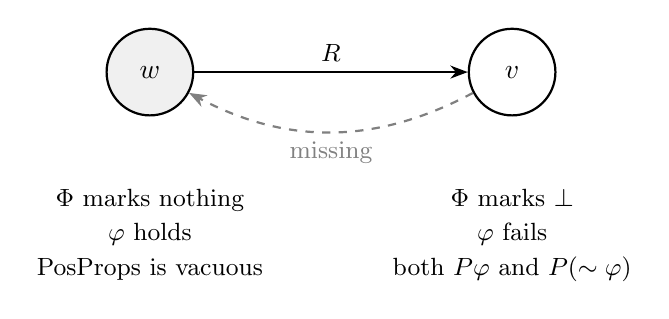
\begin{tikzpicture}[
  world/.style={circle, draw, thick, minimum size=11mm, inner sep=1pt},
  tag/.style={font=\small, align=center},
  arr/.style={-{Stealth[length=2.2mm]}, thick}
]
  \node[world, fill=black!6] (w) at (0,0) {$w$};
  \node[world] (v) at (4.6,0) {$v$};
  \draw[arr] (w) -- node[above, font=\small] {$R$} (v);
  \draw[arr, dashed, gray] (v) to[bend left=28]
    node[below, font=\small, gray] {missing} (w);
  \node[tag, below=8mm of w]
    {$\Phi$ marks nothing\\[0.15em]
     $\varphi$ holds\\[0.15em]
     $\mathrm{PosProps}$ is vacuous};
  \node[tag, below=8mm of v]
    {$\Phi$ marks $\bot$\\[0.15em]
     $\varphi$ fails\\[0.15em]
     both $P\varphi$ and $P(\sim\varphi)$};
\end{tikzpicture}
\caption{The collection used by \lean{fig7\_implies\_symmetric}.
At the source, \(\Phi\) is empty, so Ax1Gen owes nobody a positivity
premise.
At a successor that cannot see the source, the same \(\Phi\) marks the empty
property, \(\varphi\) is ``the world is the source'', and Ax4 with Ax2a
disagree.}
\label{fig:phi}
\end{figure}

\subsection{The argument}

\begin{theorem}[\lean{fig7\_implies\_symmetric}]
\label{thm:sym}
From Ax1Gen, Ax2a, Ax2b, and Ax4 it follows that \(R\) is symmetric.
Reflexivity and transitivity are not hypotheses.
\end{theorem}

\begin{proof}[Sketch]
Fix \(R\,w\,v\), and suppose \(\neg R\,v\,w\).
Define a property and a collection by
\begin{align*}
  \varphi &\;:\equiv\; \lambda\,\_\,u.\; (u = w),\\
  \Phi &\;:\equiv\; \lambda\,\psi\,u.\;
    \bigl(u \neq w \land \forall x.\; \neg\, \psi\,x\,u\bigr).
\end{align*}
At \(w\), the clause \(u \neq w\) fails, so \(\Phi\) marks no property and
\(\mathrm{PosProps}\,\Phi\) holds outright.

The boxed biconditional holds at every successor \(u\) of \(w\).
If \(u = w\), the right-hand side is vacuous and the left-hand side says that
the world is \(w\).
If \(u \neq w\), then \(\Phi\) marks \(\bot\).
The right-hand side asks \(\bot\) of an individual and is impossible, while
the left-hand side, ``the world is \(w\)'', is false.
Both sides fail together.
(The impossibility is a classical contradiction: if the world were not \(w\),
\(\bot\) would be marked and could not hold.)

Ax1Gen therefore yields \(P\,\varphi\) at \(w\).
Ax2b pushes it to \(v\).
At \(v\), necessary inclusion of \(\varphi\) in \(\sim\varphi\) is vacuous.
A successor of \(v\) cannot be \(w\), because \(v\) does not see \(w\), so the
antecedent \(\varphi\) never fires.
Ax4 yields \(P(\sim\varphi)\) at \(v\).
Ax2a says that \(P\,\varphi\) and \(P(\sim\varphi)\) are exclusive.
Contradiction.
Hence \(R\,v\,w\).
\end{proof}

Ax3 is not used.
The same four hypotheses are therefore unsatisfiable on every non-symmetric
frame.
In particular they are unsatisfiable on the two-world chain of
Figure~\ref{fig:chain}, which is the content of
\lean{fig7\_unsat\_on\_S4\_chain}.
That chain is an S4 frame.
It is not a countermodel to literal Figure~7, because no positivity and no
existence predicate satisfy the axioms there.

\begin{theorem}[\lean{th3\_fig7}]
\label{thm:th3}
From Ax1Gen, Ax2a, Ax2b, Ax3, and Ax4,
\[
  \valid{\Pos(\exE x.\, G x) \supset \Nec(\exE y.\, G y)}.
\]
There is no frame hypothesis.
\end{theorem}

\begin{proof}[Sketch]
Theorem~\ref{thm:sym} supplies symmetry.
The AFP argument then runs, as \lean{th3\_of\_symmetric}.
A diamond at \(w\) is a successor \(v\) at which some existing individual is
God-like.
Theorem Th2, which is \(G\,x \supset \Nec(\exE G)\) and which needs Ax2a, Ax2b,
and Ax3, places a God-like being at every successor of \(v\).
Symmetry puts \(w\) among them.
Th2 at \(w\) is the box required by Th3.
\end{proof}

The intermediate AFP lemmas that do not mention symmetry are in the same
file, and they are rediscoveries of the AFP proofs: \lean{lemma\_L}, the
forward spread of negative positivity \lean{ax2b'}, \lean{th1\_fig7}
(God-likeness is an essence), and \lean{th2\_fig7}.
Th4, possible existence, and Th5, necessary existence at every world, are
likewise rediscoveries for Figure~7.
Th4 is the usual indirect argument: if \(G\) were nowhere exemplified along
\(R\), then \(G\) would necessarily include \(\bot\), Ax4 would make \(\bot\)
positive, and Ax2a would refuse.
The one-world control below shows that the axioms are not jointly absurd once
a back-edge is allowed.
On a one-point frame the back-edge is the reflexive loop, so S4 and S5 agree
there.
The interesting content of Theorem~\ref{thm:th3} is the case where one tries
to withhold it.

\begin{proposition}[\lean{unit\_fig7\_th3}]
\label{prop:unit}
On a single world, with the identity relation, one individual existing there,
and principal positivity \(P\,\varphi :\equiv \varphi\,()\,()\), axioms Ax1,
Ax2a, Ax2b, Ax3, Ax4, and Ax1Gen hold, and Th3 holds.
\end{proposition}

This is the shape Nitpick reported at cardinality one, checked directly.
It is a consistency witness for the literal package.
It is not a claim that the axioms are true of anything outside the model.

\subsection{Figure 8, and what is not claimed}

Figure~8 (\lean{GoedelVariantHOML3}) changes two clauses.
Necessary inclusion gains a side condition, and essence loses the conjunct
\(\varphi\,x\):
\[
  \varphi \necImp \psi
    \;\equiv\;
    \Nec\bigl(\varphi \neq (\lambda x.\,\bot)
      \land \allE y.\, \varphi\,y \supset \psi\,y\bigr),
\]
with essence the universal closure of that inclusion under properties the
individual has.
In the Lean file the inequality is \lean{neBot}, the extensional disagreement
of Section~\ref{sec:encoding}.
The S4 theory again leaves Th3 as \lean{oops}, comment ``Open problem''.

\begin{theorem}[\lean{th3\_fig8}]
\label{thm:fig8}
From literal Ax1Gen, Ax2a, Ax2b, Figure~8's Ax3, and Figure~8's Ax4, Th3 holds,
with no frame hypothesis.
\end{theorem}

The symmetry argument is the one in Theorem~\ref{thm:sym}.
Figure~8's inclusion asks, in addition, that \(\varphi\) not be identically
false.
The witness property ``the world is \(w\)'' disagrees with \(\bot\) at \(w\),
once any individual is on hand to point at.
Theorem \lean{th3\_fig8} takes that individual from the diamond in the
antecedent of Th3, proves symmetry from it, and only then runs the back-edge.
If the type of individuals were empty the diamond could not hold, so the
implication would be idle.
The companion \lean{fig8\_implies\_symmetric} states the extra inhabitant as a
hypothesis, because symmetry alone, with no diamond, has to be told that
someone exists.
On the S4 chain, once an individual is given, the Figure~8 axioms used for
symmetry are unsatisfiable (\lean{fig8\_unsat\_on\_S4\_chain}).

Figure~8's Th4 is not claimed, and neither is a Figure~8 Th5.
The Figure~7 proof that \(G\) is possibly exemplified sends \(G\) down to
\(\bot\) and then sends \(\bot\) up to \(\sim\bot\).
For Figure~7 the second inclusion is vacuous: a false antecedent implies
anything.
Figure~8's inclusion requires the antecedent property to be distinct from
\(\bot\), and \(\bot\) is not.
In \lean{GoedelVariantHOML3.thy} the Th4 script is \lean{oops}, and Th4 is
then reintroduced by \lean{axiomatization}.
Copying that postulate into Lean would not be a proof.
It is not one here.

\subsection{Why Theorem 1 may be an accident of the abbreviation}
\label{sec:accident}

Theorem~\ref{thm:th3} is a theorem of the literal AFP axiom.
It may also be a theorem one did not mean to state.

G\"odel's footnote, as the generalized conjunction is used in this literature,
says that a conjunction of \emph{positive} properties is positive
\cite{goedel1995,benzmueller2026}.
In the abbreviation, ``the conjuncts are positive'' is judged at the source,
and ``\(\varphi\) is their conjunction'' is judged at successor worlds, where
\(\Phi\) is evaluated afresh.
The collection in Figure~\ref{fig:phi} is empty at home and full of
contradictions next door.
Nothing in the footnote asks a collection to change its mind on the way out
of the world.
The split is what a shallow embedding does if \(\mathrm{PosProps}\) is left
outside a box while the predicate \(\Phi\) still depends on the world.

That is a feature of the definition as written in
\lean{GoedelVariantHOML2}.
It is a fair question whether it is a feature anyone wanted.
Theorem~\ref{thm:th3} would be a strange place to stop.
The next section is the reason for not stopping: two repairs that a reader
of the footnote might have thought were already the axiom.
Under either repair, lemma~L survives, symmetry is not forced, and Th3 fails
in S4.

\section{Theorem 2: repair the scope, and S4 wins}
\label{sec:th2}

Everything in Figure~7 stays put except Ax1Gen.
There are two replacements.
They are not rivals for a single idea.

\paragraph{R1, positivity in the box.}
The closer repair judges both halves at the same accessible worlds:
\[
  \valid{\Nec\bigl(\mathrm{PosProps}\,\Phi \land
    \allE z.\; \varphi\,z \leftrightarrow
    (\forall \psi.\; \Phi\,\psi \supset \psi\,z)\bigr)
    \supset P\,\varphi}.
\]
Call this \lean{Ax1GenInBox}.
In~K, a box of a conjunction is a conjunction of boxes, and
ConjOfPropsFrom is already a box, so the displayed form is equivalent to
\[
  \valid{(\Nec(\mathrm{PosProps}\,\Phi) \land
    \mathrm{ConjOfPropsFrom}\,\varphi\,\Phi) \supset P\,\varphi},
\]
which is \lean{Ax1GenBox}.
The equivalence \lean{ax1GenBox\_iff\_inBox} depends on no kernel axioms.
One countermodel covers both spellings.
This is the reading on which ``positive'' and ``conjunction'' are said of the
same world.

\paragraph{R2, a rigid collection.}
Restrict Ax1Gen to collections that do not depend on the world:
\(\Phi\,\psi\,w \leftrightarrow \Phi\,\psi\,v\) for every property and every pair of
worlds.
PosProps and ConjOfPropsFrom stay literal.
Call this \lean{Ax1GenRigid}.
The prank collection of Figure~\ref{fig:phi} is not rigid, so R2 never sees it.
R2 is a different restriction, not a second spelling of R1.

\subsection{Lemma L still derives}

Under R1, lemma~L is immediate from the repaired axiom alone
(\lean{lemma\_L\_box}, \lean{lemma\_L\_inBox}).
Take \(\Phi\) to be \(P\) itself.
At every world, every property that \(\Phi\) marks is positive there, by
identity, so the extra box is free.
The conjunction of whatever is positive at a world is \(G\) at that world, by
the definition of \(G\).

Under R2 the same \(\Phi\) may be refused, because \(P\) itself need not be
rigid.
The repair is to take a snapshot at the world \(w\) where the lemma is being
proved: \(\Phi\,\psi\,\_ :\equiv P\,\psi\,w\).
That collection ignores its world argument, so it is rigid.
At a successor \(v\), the conjunction it defines is \(G\) only if positivity at
\(w\) and positivity at \(v\) agree.
Ax2a and Ax2b give exactly that agreement along an edge
(\lean{pos\_agree}): a positive property stays positive by Ax2b, and a
property positive at \(v\) cannot have a positive negation at \(w\), or Ax2b
would carry the negation forward and break Ax2a at \(v\).
So \lean{lemma\_L\_rigid} needs Ax2a and Ax2b.
Literal \lean{lemma\_L} needed neither.
The box in R1 hides the same fact, because \(\Phi := P\) is re-read at the
successor rather than frozen at the source.

Symmetry is not a consequence of either repair.
The collection in Theorem~\ref{thm:sym} is empty at the source, so source
PosProps holds, but at a successor it marks \(\bot\).
R1's boxed PosProps demands \(P(\bot)\) there.
R2 does not apply, because the collection varies.
The four-hypothesis derivation of a back-edge has nothing left to instantiate.

\subsection{The chain}

\begin{figure}[t]
\centering
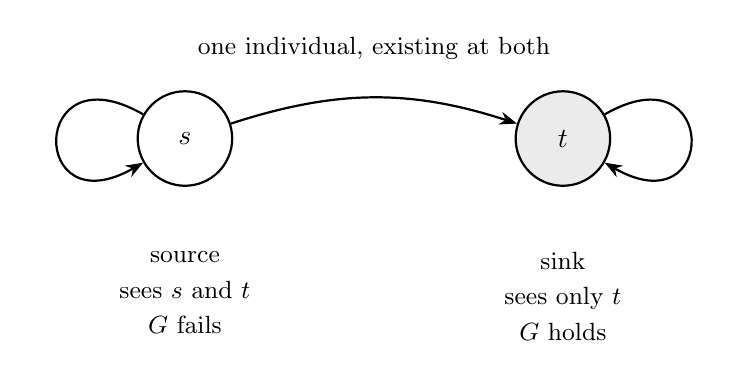
\begin{tikzpicture}[
  world/.style={circle, draw, thick, minimum size=12mm, inner sep=1pt},
  tag/.style={font=\small, align=center},
  arr/.style={-{Stealth[length=2.2mm]}, thick}
]
  \node[world] (s) at (0,0) {$s$};
  \node[world, fill=black!8] (t) at (4.8,0) {$t$};
  \draw[arr] (s) to[out=150,in=210,looseness=7] (s);
  \draw[arr] (t) to[out=30,in=-30,looseness=7] (t);
  \draw[arr] (s) to[bend left=18] (t);
  \node[tag, below=7mm of s]
    {source\\[0.2em]
     sees \(s\) and \(t\)\\[0.2em]
     \(G\) fails};
  \node[tag, below=7mm of t]
    {sink\\[0.2em]
     sees only \(t\)\\[0.2em]
     \(G\) holds};
  \node[tag] at (2.4,1.15) {one individual, existing at both};
\end{tikzpicture}
\caption{The S4 chain of \lean{R\_chain}, drawn as source \(s = \mathsf{false}\)
and sink \(t = \mathsf{true}\).
Reflexive, transitive, and not symmetric.
Under \lean{chainP}, a God-like being exists at the sink only, so at the
source a God-like being is possible and not necessary.
Literal Ax1Gen has no model on this frame.
Both repairs do.}
\label{fig:chain}
\end{figure}

Let the worlds be the two Booleans.
The source \(\mathsf{false}\) sees both worlds.
The sink \(\mathsf{true}\) sees only itself
(Figure~\ref{fig:chain}).
The relation is reflexive and transitive.
It is not symmetric: the sink does not see the source.
One individual exists at both worlds.
Positivity ignores the world at which it is asked and reads the sink:
\[
  P\,\varphi \;\equiv\; \varphi\,()\,\mathsf{true}.
\]
A property is positive precisely when the individual has it at \(t\).

At the sink, God-likeness is a tautology.
\(G\) says that every positive property holds of the individual there, and
positivity means that the property holds of the individual there
(\lean{chain\_god\_sink}; no kernel axioms).
At the source it fails.
The property ``the world is the sink'' holds at the sink, hence is positive,
and the individual does not have it at the source
(\lean{chain\_not\_god\_source}; no kernel axioms).

\begin{theorem}[\lean{chain\_th3\_fails\_at\_source}]
\label{thm:fails}
At the source, \(\Pos(\exE G)\) holds and \(\Nec(\exE G)\) fails.
\end{theorem}

\begin{proof}[Sketch]
The source sees the sink, where the individual exists and is God-like.
The source also sees itself, where that same individual exists and is not
God-like.
The diamond is the first fact.
The failure of the box is the second.
\end{proof}

No kernel axiom is used.
The packaged denial \lean{chain\_not\_Th3} is the same fact pulled back along
the definition of Th3, and it is equally axiom-free.

\begin{theorem}[\lean{r1\_s4\_countermodel}, \lean{r2\_s4\_countermodel}]
\label{thm:r12}
On this frame the relation is an S4 frame and not a symmetric one.
Ax1, Ax2a, Ax2b, Ax3, Ax4, and both spellings of R1 hold, and Th3 fails.
The same frame, the same positivity, and the same existence predicate satisfy
R2, and Th3 fails.
\end{theorem}

The axiom checks are direct, and most of them use no kernel axioms.
Ax2a is the exclusive-or of ``\(\varphi\) holds at the sink'' and ``\(\varphi\)
fails at the sink'', which is classical excluded middle
(\lean{chain\_ax2a}).
Ax2b is immediate because \(P\) does not look at its world argument: positivity
is already global.
Ax4 follows because both worlds see the sink, so a necessary inclusion can be
read there, where \(P\) evaluates extensions.
Ax3 holds because \(P\) on necessary existence only asks for the extension at
the sink, and the essence hypothesis at the sink includes that the property
holds of the individual there.
For R1, the boxed biconditional at whichever world one starts from can be read
at the sink, which both worlds see, and the right-hand side at the sink is
exactly the extension \(P\) consults.
For R2 the same computation works, and rigidity lets a mark at the sink be
copied back to the world where PosProps was assumed.

\begin{proposition}[\lean{chain\_not\_literal\_Ax1Gen}]
This positivity does not satisfy literal Ax1Gen on the chain.
\end{proposition}

If it did, Theorem~\ref{thm:sym} would make the chain symmetric, and
\lean{fig7\_unsat\_on\_S4\_chain} already records that contradiction.
The repairs are strictly weaker than the literal axiom on this frame.
Theorem~\ref{thm:th3} is not retracted.
It is fenced.
A model of R1 or of R2 need not be a model of the abbreviation that proved it.

\begin{table}[t]
\centering
\small
\begin{tabular}{@{}lccc@{}}
\toprule
Reading of Ax1Gen & Lemma \(P(G)\) & Symmetry forced & Th3 in S4 \\
\midrule
Literal AFP &
  from Ax1Gen alone &
  yes (Thm.~\ref{thm:sym}) &
  proved (Thm.~\ref{thm:th3}) \\
R1, boxed &
  from R1 alone &
  no &
  fails (Thm.~\ref{thm:r12}) \\
R2, rigid \(\Phi\) &
  needs Ax2a and Ax2b &
  no &
  fails (Thm.~\ref{thm:r12}) \\
\bottomrule
\end{tabular}
\caption{The S4 question, by scope.
The witness for both negative cells is Figure~\ref{fig:chain}.}
\label{tab:readings}
\end{table}

Table~\ref{tab:readings} is the whole comparison.
The possibilist twin \lean{GoedelVariantHOML2possInS4} also leaves Th3 as
\lean{oops}.
It is not encoded.
A constant domain with no existence predicate would be a different theorem,
and the Scott-style chain already studied in this repository is that
different theorem (Section~\ref{sec:related}).

\section{What was already known}
\label{sec:related}

Several nearby statements are in the same repository, and they were already
theorems of other people.
They are named here so that the two results above are not asked to carry them.

Sobel showed that Scott-style premises yield \(\varphi \supset \Nec\varphi\)
\cite{sobel1987,sobel2004}.
Benzm\"uller and Fuenmayor encoded Scott's, Anderson's, and Fitting's
variants and checked that Scott's intensional positivity collapses modality,
while Anderson's emendation and Fitting's extensional positivity do not
\cite{benzmuellerFuenmayor2020,anderson1990,andersonGettings1996,fitting2002}.
The repository's collapse modules rediscover the Scott-side collapse, including
the world-relative variant in which collapse along \(R\) is separated from
Sobel's global biconditional when \(R\) is not universal.
That is a rediscovery.
It is not Theorem~\ref{thm:th3} or Theorem~\ref{thm:r12}.

Kanckos and Woltzenlogel Paleo showed that Scott's argument goes through in KB:
symmetry suffices, and S5 is more than the proof uses \cite{kanckos2017}.
Benzm\"uller and Scott make the same point for their Th3, which cites
\(R_{\mathrm{symm}}\) and not reflexivity or transitivity
\cite{benzmuellerScott2025,afpNotes2025}.
The repository's Scott-style development rediscovers the positive half
(local Th3 from symmetry alone, on that encoding) and pairs it with
countermodels once symmetry is dropped.
Those countermodels postulate positivity of being God-like.
Figure~7 derives that sentence as lemma~L.
A countermodel that assumes the lemma does not answer a question whose point
is what happens when the lemma is earned from Ax1Gen.
The file \lean{S4Open.lean} in the repository is an explicit record of this
mismatch.
Theorem~\ref{thm:r12} is not that countermodel.
On the chain of Figure~\ref{fig:chain} the literal axiom has no model at all.

Anderson's emendation---only one direction of the exclusion axiom, and
God-likeness as possession of exactly the positive properties, necessarily---is
a known repair \cite{anderson1990,andersonGettings1996}.
A thin fragment of it is formalized elsewhere in the repository, and a
two-world witness there keeps a contingent fact alive.
That fragment is a rediscovery of Anderson's repair.
Fitting's extensional block is not formalized \cite{fitting2002}.
Neither is part of Theorems~\ref{thm:th3} and~\ref{thm:r12}.

The early mechanizations of the Scott-style argument
\cite{benzmuellerPaleo2014} are the same Scott package.
Benzm\"uller's note on ultrafilters \cite{benzmueller2026} derives
\(\valid{\Nec(\exE x.\, G x)}\) already in K, from an ultrafilter axiom U1, a
conjunction principle, an entailment axiom, and the definition of \(G\).
The note is explicit that this is a simplified package, and that Scott's own
A3 postulated \(P(G)\) in place of the footnote's conjunction.
It is not Figure~7's axiom list, and it does not use the AFP scoping of
Ax1Gen.
The Archive entry on simplified variants \cite{afpSimplified2021} studies
arguments that avoid essence and necessary existence and that are valid in K
or KT.
Those are different axioms again.

What was checked, for the claim that these two theorems were not found
already, is the following AFP theories, together with the S4 and S5 embeddings
they import:
\begin{itemize}[leftmargin=1.5em]
\item \lean{GoedelVariantHOML2} and \lean{GoedelVariantHOML2inS4} (Figure~7, S5 and S4);
\item \lean{GoedelVariantHOML3} and \lean{GoedelVariantHOML3inS4} (Figure~8, S5 and S4);
\item \lean{GoedelVariantHOML2possInS4} (the possibilist S4 twin, not encoded here).
\end{itemize}
The literature named in this section was checked as well, namely the items
cited from the repository notes that accompany the formalization:
Sobel
\cite{sobel1987,sobel2004}, Anderson \cite{anderson1990}, Anderson and Gettings
\cite{andersonGettings1996}, Fitting \cite{fitting2002}, Kanckos and
Woltzenlogel Paleo \cite{kanckos2017}, Benzm\"uller and Woltzenlogel Paleo
\cite{benzmuellerPaleo2014}, Benzm\"uller and Fuenmayor
\cite{benzmuellerFuenmayor2020}, Benzm\"uller \cite{benzmueller2026}, and the
simplified-argument AFP entry \cite{afpSimplified2021}.
In the AFP S4 files, Th3 is the open \lean{oops}.
In \cite{benzmueller2026} the K-theorem is the ultrafilter package just
described.
No proof or countermodel of literal Figure~7 Th3 in S4, and no countermodel
of the two repaired readings, turned up in those sources.
That is a statement about where the search went.
It is not a priority claim.

\section{What the kernel accepts}
\label{sec:kernel}

The development builds with \texttt{lake build} on Lean~4.34.0,
toolchain \texttt{leanprover/lean4:v4.34.0}, in 35 jobs, with no Mathlib.
A search of the Lean sources finds no \lean{sorry}, no \lean{native\_decide},
and no \lean{axiom} command.
The strings that look like those words sit in comments.
Hypotheses of the ontological argument are parameters of type \textsf{Prop}.

Table~\ref{tab:axioms} is the output of \lean{\#print axioms} on the headline
theorems, run in that toolchain after the build.
``None'' means Lean reported that the constant does not depend on any axioms.
The triple \lean{propext}, \lean{Classical.choice}, \lean{Quot.sound} is the
standard classical package of the Lean kernel: propositional extensionality,
choice, and the soundness of quotients that the classical development uses.
\lean{Classical.choice} enters through \lean{Classical.byContradiction} in the
symmetry argument and in Figure~7's Th4, and through \lean{Classical.em} in
the one-world check of Ax2a and in \lean{chain\_ax2a}.
\lean{propext} on its own is the chain's transitivity and the proof that the
chain is not symmetric, both of which simplify propositional equalities.
No custom axiom appears.

\begin{table}[t]
\centering
\footnotesize
\begin{tabular}{@{}>{\raggedright\arraybackslash}p{0.56\textwidth}>{\raggedright\arraybackslash}p{0.38\textwidth}@{}}
\toprule
Theorem & \lean{\#print axioms} \\
\midrule
\lean{lemma\_L}, \lean{ax2b'}, \lean{th1\_fig7}, \lean{th2\_fig7},
  \lean{th3\_of\_symmetric} &
  none \\
\lean{th1\_fig8}, \lean{th2\_fig8}, \lean{th3\_fig8\_of\_symmetric} &
  none \\
\lean{fig7\_implies\_symmetric}, \lean{th3\_fig7},
  \lean{fig7\_unsat\_on\_S4\_chain} &
  \lean{propext}, \lean{Classical.choice}, \lean{Quot.sound} \\
\lean{th3\_fig8}, \lean{fig8\_implies\_symmetric},
  \lean{fig8\_unsat\_on\_S4\_chain} &
  \lean{propext}, \lean{Classical.choice}, \lean{Quot.sound} \\
\lean{unit\_fig7\_th3} &
  \lean{propext}, \lean{Classical.choice}, \lean{Quot.sound} \\
\lean{ax1GenBox\_iff\_inBox} &
  none \\
\lean{lemma\_L\_box}, \lean{lemma\_L\_inBox}, \lean{lemma\_L\_rigid} &
  none \\
\lean{chain\_th3\_fails\_at\_source} &
  none \\
\lean{chain\_not\_literal\_Ax1Gen} &
  \lean{propext}, \lean{Classical.choice}, \lean{Quot.sound} \\
\lean{r1\_s4\_countermodel}, \lean{r2\_s4\_countermodel} &
  \lean{propext}, \lean{Classical.choice}, \lean{Quot.sound} \\
\bottomrule
\end{tabular}
\caption{Kernel axioms of the headline theorems, Lean~4.34.0.
The repaired countermodels inherit \lean{propext} from the chain's frame
facts and \lean{Classical.choice} from Ax2a.
The failure of Th3 at the source, taken by itself, depends on none of them.}
\label{tab:axioms}
\end{table}

\section{The moral}

Theorem~\ref{thm:th3} says that the literal Figure~7 axioms prove Th3, and
prove it in K, hence in S4.
The mechanism is the empty-at-home collection of Figure~\ref{fig:phi}, which
the AFP abbreviation permits because positivity is read at the source and the
collection is read again under the box.
Theorem~\ref{thm:r12} says that if positivity moves inside the box, or if the
collection is required to be the same collection at every world, then lemma~L
still derives and the two-world chain is a countermodel to Th3 in S4.
The chain does not satisfy the literal axiom.
The S4 question, for this axiom list, is decided by that scope and by nothing
else in the modal logic.

\section*{Acknowledgements}

The Lean~4 formalization and the drafting of this note were done with AI
coding assistants.
All results reported here are kernel-checked in the repository
\url{https://github.com/drewarrowood/godel-ontological}.

\bibliographystyle{plain}
\bibliography{refs}

\end{document}
